\section{Modèle théorique de Mumford Shah}

Ce modèle est l'un des plus étudié. La fonctionnelle de Mumford-Shah a été introduite en 1989. D'un point de vue continue, une image est vue comme une fonction $g : \Omega \rightarrow \mathbb{R}$, où $^Omega$ est par exemple un rectangle, et $g$ associe à chaque point $x \in \Omega$ de l'image une valeur $g(x)$ qui représente un niveau de gris. La fonction g n'est pas régulière, elle est très souvent discontinue. c'est cet effet de discontinuité qui nous intéresse. En effet, nous voulons trouver pour une image $g : \Omega \rightarrow \mathbb{R}$ l'ensemble des contours des objets que représente l'image. Ces contours sont dont localisés au points de discontinuités de g : il y a une franche discontinuité dans les niveaux de gris.

Pour résoudre ce problème, Mumford et Shah introduisent une fonctionnelle qui par minimisation, va chercher les points de $g$ les plus discontinus. \\

Le problème s'écrit alors : 
\[\underset{(u, K) \in \mathcal{A}(\Omega)}{min} \; \; \; J(u,K) := \int_{\Omega \backslash K} |u - g |^2 dx + \int_{\Omega \backslash K} ||\nabla u ||^2 dx + \mathcal{H}^1(K) ,  \]

avec 
\[ \mathcal{A} (\Omega) = \{ (u,K) : K \subset \Omega \; \; \; \text{est fermé et } \; \; \; u \in C^1(\Omega \backslash K) \} \] 

Nous pouvons expliciter chacun des termes qui composent cette fonctionnelle :\\

$ - \int_{\Omega \backslash K} |u - g |^2 dx $ force u, par minimisation, à ressembler le plus possible à l'image de départ g. \\

$ - \int_{\Omega \backslash K} ||\nabla u ||^2 dx $ pénalise les oscillations de u, qui par minimisation, forcera u a être la plus régulière possible. Comme g est très irrégulière au début, on ne peut pas avoir $ u = g$ partout dans $\Omega$. Ainsi, l'ensemble K possède un rôle essentiel : s'il est bien positionné sur les singularités de $g$, il permettra de minimiser le premier terme décrit ci-dessus.\\

$ - \mathcal{H}^1(K) $ désigne la mesure de Hausdorff de dimension 1 de l'ensemble $K$. Ce dernier terme force $K$ à être de dimension de Hausdorff $1$, qui nous donne bien l'intuition d'un "contour". Par exemple, un cercle est de dimension de Hausdorff 1. Cet ensemble $K$ devra être optimisé pour couvrir le plus possible les singularités de $g$, en le positionnant en priorité sur les discontinuités les plus franches. Les autres singularités non prise en compte dans ce terme, donc minimes, seront considérés en oscillations. $\mathcal{H}^1(K)$ est la mesure de Lebesgue sur $\mathbb{R}$.\\


\subsection{Mesure et dimension de Hausdorff : compléments}
Les mesures de Hausdorff sont une généralisation des notions de longueur, d'aire, de volume... $\mathcal{H}^n$ est la mesure de Lebesgue en dimension $n$ pour des sous ensembles de $\mathbb{R}^n$, multipliée par une constante qui n'est autre que le volume $n-dimensionel$ de la boule unité. \\

La mesure de Hausdorff peut être définie pour tout ensemble. Pour un sous-ensemble non-vide $U$ d'un espace euclidien de dimension $n$, on peut définir le diamètre de $U$ tel que : 

\[ diam \; \; U  =  |U| = sup\{ |x-y| \;  :  \; x,y \in U \}\] 
Avec la distance euclidienne usuelle.\\

Ensuite, si un ensemble F est recouvert par une collection dénombrable $\{U_i\}$, de diamètre au plus $\delta$ : 

\[ F = \cup_{i=1}^{\infty} U_i \; \; \; \text{avec}\; \; \; 0 < |U_i| \leq \delta  \]
 On dit que $\{U_i\}$ est un $\delta$-recouvrement de $F$. \\
 
Soit maintenant un $s \in \mathbb{R} >0 $. Pour tout $\delta >0$, on peut définir : 

\[ \mathcal{H}_{\delta}^s (F) = inf \{ \sum \limits_{i=1}^{\infty} |U_i|^s \; : \; \{U_i\} \text{est un recouvrement de } F\}\].

Ainsi, 

\[ \mathcal{H}^s (F) = \underset{\delta -> 0}{lim} \mathcal{H}_{\delta}^s (F)\] 

Et $\mathcal{H}^s (F)$ est appelé la mesure de Hausdorff s-dimensionnelle de $F$. \\

$\textit{Théorème 1 : Dimension de Hausdorff (admis)}$ : Soit $F$ un sous-ensemble. Il existe un unique  $d \in \mathbb{R}_{+} \cup {\infty}$ tel que : 
\[ 1. \; \; \mathcal{H}^s (F) = \infty \; \; \; \text{pour tout} \; \;  s<d \] 
\[ 2. \; \; \mathcal{H}^s (F) = 0 \; \; \; \text{pour tout} \; \; s>d \] 

On appelle dimension de Hausdorff de $F$ le réel $d$. C'est la valeur critique de s pour laquelle la mesure passe de $0$ à $\infty$ \\

On l'appelle également dimension fractale. 

\begin{figure}[H]
\centering
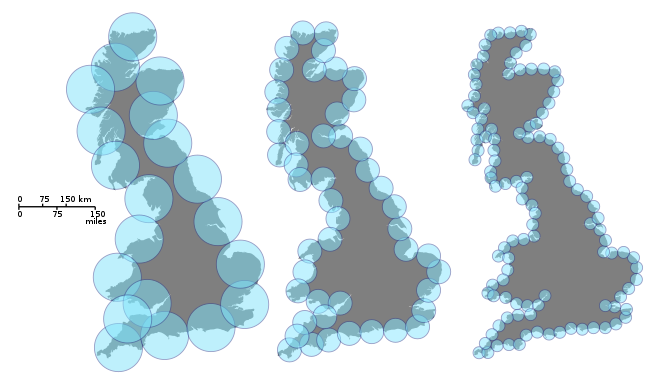
\includegraphics[scale=0.5]{../../images/hausdorff.png}
\caption{Dimension de Hausdorff de la Grande Bretagne }
\end{figure}



\section{Modèle discret et implémentation numérique}

On veut minimiser en $\Omega \subset \{1,...,N\}^2$ et en $w \in \mathbb{R}^{N^2}$ la fonctionnelle : 

\[ P(\Omega) + \lambda \sum \limits_{\underset{((m,n), (m, n+1)) \notin \partial \Omega}{\underset{((m,n),(m+1, n)) \notin \partial \Omega}{m,n = 1}}}^{N} |\nabla w_{m,n}|^2 + \mu ||w - u ||_2^2 \]

où $\lambda \geq 0$, $\mu \geq 0$ sont des paramètres et $u \in \mathbb{R}^{N^2}$ est l'image à segmenter. Pour cela, on va utiliser un algorithme de descente sur $\Omega$ et $w$. \\

Le premier terme de la somme est très proche d'un terme $H^1$, sauf que l'on retire de la somme les points dont le calcul du gradient fait intervenir un voisin de l'autre côté de la frontière de $\Omega$. Ainsi, les points qui ont un très fort gradient tendent à appartenir à la frontière. Le dernier terme constitue l'attache au données. 
\subsection{Notion de périmètre}
On veut minimiser le terme correspondant au périmètre de $\Omega$. Pour définir ce périmètre, on considère un système de voisinage $\delta(m,n)$ de chaque pixel $(m,n) \in \{1,...,N\}^2$. Les voisinages les plus utilisés sont la 4-connexité définie comme ci dessous :

\[ \sigma (m,n) = \{ (m',n') \in  \{1,...,N\}^2, |m - m' | + |n - n'| = 1 \}\]
Ou la 8-connexité définie comme ci dessous : 
\[ \sigma (m,n) = \{ (m',n') \in  \{1,...,N\}^2, max(|m - m' | , |n - n'| ) = 1 \}\]

\begin{figure}[H]
\centering
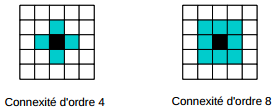
\includegraphics[scale=1]{Connexite.png}
\caption{4-connexité et 8-connexité \newline  https://ensiwiki.ensimag.fr/index.php?title=Fichier:Connexite.png}
\end{figure}

On définit alors la frontière de $\Omega \subset \{ 1,...,N\}^2$ comme l'ensemble : 
\[ \partial \Omega = \{ ((m,n),(m',n')) \in (\{ 1,...,N\}^2)^2, (m',n') \in \sigma (m,n) \; et \; (m,n)\in \Omega \; et \; (m',n') \notin \Omega \}\] 

Le périmètre de $\Omega$ est alors définie par : 

\[ P(\Omega) = \sum \limits_{((m,n),(m',n')) \in \partial \Omega} dl((m,n),(m',n')),\] 

Où $ dl((m,n),(m',n')) > 0$ sont des éléments de longueur. Plus la frontière de $\Omega$ contient d'éléments, plus la longueur du contour sera grande. On suppose également pour simplifier que pour tout $((m,n), (m',n')) \in (\{ 1,...,N\}^2)^2$ 

\[ dl((m,n),(m',n')) = dl((m',n'),(m,n))\].

On suppose aussi que 
\[ \text{si} \; (m',n') \notin \sigma (m,n) \; \; \; \text{alors} \; \; dl((m,n),(m',n')) = 0\]

Pour optimiser $\Omega$, on va procéder par des ensemble de niveau. 
\subsubsection{Représentation de $\Omega$}
Les méthodes basées sur les ensembles de niveaux représentent l'ensemble $\Omega \subset \{1,...N\}^2$ comme un ensemble de niveau d'une image $\phi \in \mathcal{R}^{N^2}$. On pose donc 

\[ \Omega = \{ (m,n) \in \{1,...,N \}^2, \phi_{m,n} \geq 0 \} \].
\subsubsection{Evolution de $\Omega$}
Ainsi, faire évoluer $\Omega$ revient à faire évoluer l'image $\phi$ pour minimiser une énergie analogue mais portant sur $\phi$. On applique un algorithme de gradient à la fonctionelle. On peut donc construire une énergie en $\phi$ tel que : 

\[ E ((\phi_{m,n})_{1 \leq m,n \leq N}) = \sum \limits_{m,n = 0}^N  \sum \limits_{m',n' = 0}^N  dl((m,n),(m',n')) H_{\epsilon} (\phi_{m,n}) ( 1 - H_{\epsilon}(\phi_{m',n'})) \] 
Avec 
\[ H_{\epsilon} (t) = \left\{ \begin{matrix}
1 & \text{si} \; t \geq \epsilon \\
\frac{1}{2} (1 + \frac{t}{\epsilon} + \frac{1}{\pi}sin(\frac{\pi t}{\epsilon})) & \text{si} -\epsilon \leq t \leq \epsilon \\
0 & \text{si} t \leq - \epsilon 
\end{matrix} \right. \] 
Ainsi que son gradient en $\phi = (\phi_{m,n})_{1 \leq m,n \leq N}$ : 

\[ \nabla E (\phi) = ( \sum \limits_{m',n' = 0}^N dl((m,n),(m',n')) H_{\epsilon}' (\phi_{m,n}) ( 1 - 2H_{\epsilon}(\phi_{m',n'})) ) _{1 \leq m,n \leq N}  \] 

Avec 
\[ H_{\epsilon}' (t) = \left\{ \begin{matrix}
0 & \text{si} \; t \geq \epsilon \\
\frac{1}{2 \epsilon} + \frac{1}{2 \epsilon} cos(\frac{\pi t}{\epsilon}) & \text{si} -\epsilon \leq t \leq \epsilon \\
0 & \text{si} t \leq - \epsilon 
\end{matrix} \right. \] 


Ainsi, on combine alors une étape de minimisation d'une énergie sur w, puis d'une étape d'optimisation de la forme $\Omega$. 
\subsection{Convergence de l'algorithme}
\subsection{Implémentation numérique et résultats}
